\documentclass[10pt,letterpaper]{article}
\usepackage[margin=0.72in]{geometry}
\usepackage[T1]{fontenc}\usepackage{lmodern,microtype,amsmath,amssymb,xcolor}
\usepackage[hidelinks]{hyperref}\usepackage{titlesec,enumitem,fancyhdr,tikz}
\usetikzlibrary{arrows.meta,positioning}
\definecolor{ink}{HTML}{153A50}\definecolor{accent}{HTML}{276C90}
\setlength{\parindent}{0pt}\setlength{\parskip}{5pt}
\setlist[itemize]{leftmargin=1.4em,itemsep=3pt,topsep=3pt}
\setlist[enumerate]{leftmargin=1.5em,itemsep=3pt,topsep=3pt}
\titleformat{\section}{\large\bfseries\color{ink}}{\thesection.}{0.5em}{}
\titleformat{\subsection}{\normalsize\bfseries\color{accent}}{\thesubsection}{0.5em}{}
\titlespacing*{\section}{0pt}{9pt}{4pt}\titlespacing*{\subsection}{0pt}{6pt}{3pt}
\pagestyle{fancy}\fancyhf{}\renewcommand{\headrulewidth}{0pt}
\fancyfoot[L]{\footnotesize PHYSICS 621 | Andre and Colin}\fancyfoot[R]{\footnotesize\thepage}

\begin{document}
\begin{center}
{\LARGE\bfseries\color{ink} Interference rejection and precision limits\\[3pt] in intensity-coded FMCW LiDAR}\\[6pt]
{\large Andre and Colin}\\[3pt]
{\small PHYSICS 621 | Combined project proposal | Computational design}
\end{center}
{\color{accent}\rule{\linewidth}{0.7pt}}
\section{System choice and core question}
We propose a Python simulation of a 1550-nm, single-point FMCW LiDAR measuring a stationary industrial surface while light from one independent LiDAR enters its receiver. The source follows the hybrid silicon-nitride/lithium-niobate, self-injection-locked laser architecture of Snigirev et al. \cite{snigirev}. A separate Mach--Zehnder intensity modulator (MZM) adds an identifying RF-subcarrier code. A local oscillator (LO) tapped before the MZM mixes with the delayed target return in a balanced coherent receiver. The nominal range is 50 m; 10 to 100 m is a sensitivity range, not a demonstrated operating specification.

\textbf{Core question: At fixed average launched power, acquisition time and receiver bandwidth, when does intensity coding reduce interference-induced range errors, and how do MZM bias and drive amplitude change the benefit?}

The coding idea is motivated by Hai et al. \cite{hai}, whose coded phase-shift ranging is a different measurement architecture. Transferring that idea to optical FMCW with coherent detection is our hypothesis, not an established result from either paper. A negative result, identifying when coding losses exceed interference rejection, is a useful project outcome. Chirp calibration is retained as a controlled supporting subsystem. A separate optimisation of calibration versus wider sweeps is outside the core scope.

\section{Architecture and optical flow}
\begin{center}
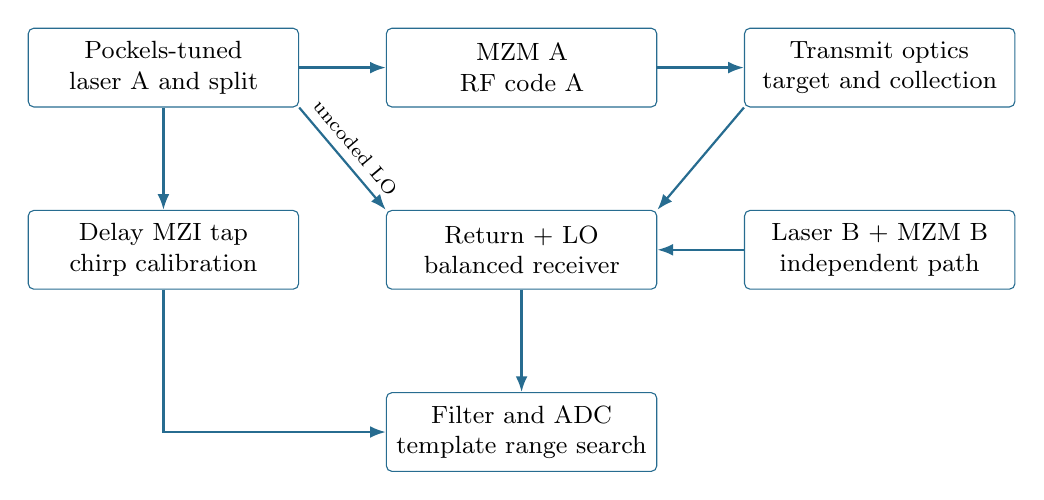
\begin{tikzpicture}[font=\small,box/.style={draw=accent,rounded corners=2pt,align=center,minimum height=10mm,text width=32mm},arr/.style={-{Latex[length=2mm]},thick,draw=accent}]
\node[box] (a) {Pockels-tuned\\laser A and split};
\node[box,right=11mm of a] (m) {MZM A\\RF code A};
\node[box,right=11mm of m] (t) {Transmit optics\\target and collection};
\node[box,below=13mm of a] (cal) {Delay MZI tap\\chirp calibration};
\node[box,below=13mm of m] (rx) {Return + LO\\balanced receiver};
\node[box,below=13mm of t] (b) {Laser B + MZM B\\independent path};
\node[box,below=13mm of rx] (dsp) {Filter and ADC\\template range search};
\draw[arr] (a)--(m);\draw[arr] (m)--(t);
\draw[arr] (a)--(cal);
\draw[arr] (a.south east)--node[above,sloped,font=\scriptsize]{uncoded LO}(rx.north west);
\draw[arr] (t.south west)--(rx.north east);
\draw[arr] (b)--(rx);\draw[arr] (rx)--(dsp);
\draw[arr] (cal.south)|-(dsp.west);
\end{tikzpicture}
\end{center}
The Pockels effect changes resonator index and the locked laser frequency. The MZM changes the transmitted field amplitude, with a nonlinear voltage-to-field transfer. Propagation adds attenuation, delay and target phase; diffuse reflection can cause speckle. The independent interferer has its own frequency offset, sweep slope, phase noise and arrival time. Optical mixing converts the returned fields into electrical beats. An optical filter limits background; a finite-bandwidth electrical filter precedes sampling. Processing compares the measurement with delayed templates for A, using the calibrated chirp and MZM response.

The unequal-arm Mach--Zehnder \emph{interferometer} (MZI) measures chirp; the Mach--Zehnder \emph{modulator} (MZM) encodes intensity. They are distinct devices. We exclude scanning, velocity estimation, chip fabrication, combs and general multi-user cancellation. One desired target and one interfering transmitter keep the project feasible for a 5 to 8 page manuscript.
\newpage
\section{Field model and course connections}
\textbf{Source and waves in materials.} For transmitter $i\in\{A,B\}$,
\begin{equation}
\nu_i(t)=\nu_{0,i}+S_it+\delta\nu_i(t),\qquad
E_{i,0}(t)=\sqrt{P_{i,0}}\exp\!\left[i2\pi\int_0^t\nu_i(u)\,du+i\phi_{n,i}(t)\right].
\end{equation}
$\delta\nu_i$ is deterministic chirp error; $\phi_{n,i}$ is stochastic phase. The guided mode overlaps LiNbO$_3$, giving approximately
\begin{equation}
\Delta n_{\rm eff}\simeq-\tfrac12\Gamma n^3r_{\rm eff}V/d,\qquad
\Delta\nu\simeq-(\nu_0/n_g)\Delta n_{\rm eff}.
\end{equation}
Modal overlap $\Gamma$, electrode spacing $d$, tensor orientation and propagation loss connect material properties to tuning and available power. A representative 28-MHz/V coefficient \cite{snigirev} would require about 18 V peak-to-peak for our assumed 0.5-GHz sweep; locking range and driver response must still be checked. This is an architectural model, not a full chip simulation.

\textbf{Nonlinear optics and modulation.} The Pockels effect arises from $P^{(2)}(\omega)\propto\epsilon_0\chi^{(2)}(\omega;\omega,0)E_{\rm opt}E_{\rm RF}$. It is linear in applied voltage but involves nonlinear material polarisation. The MZM's cosine transfer is interferometric; its distortion alone is not evidence of nonlinear optical material physics. For an ideal chirp-free, push-pull MZM,
\begin{equation}
E_{i,t}(t)=\sqrt{\eta_M}E_{i,0}(t)a_i(t),\quad
 a_i(t)=\cos\!\left[\frac{\pi}{2V_\pi}\{V_{b,i}+V_{m,i}c_i(t)\cos(2\pi f_ct)\}\right].
\end{equation}
Here $c_i(t)\in\{-1,+1\}$ is a known code with finite-bandwidth transitions, $\eta_M$ is insertion transmission, and $V_\pi$ is the differential half-wave voltage. This expression assumes a specified voltage convention and negligible residual MZM phase chirp. The launched average power is $\bar P_t=\eta_M P_{i,0}\langle a_i^2\rangle$. Retain the sign of $a_i$ in coherent detection; using $\sqrt{P_{i,t}}$ alone discards possible $\pi$ phase reversals. Bias near a null can also eliminate intensity discrimination between opposite drive signs, so deeper drive is not automatically better.

\textbf{Optical systems and detection.} Write $E_{A,r}(t)=h_AE_{A,t}(t-\tau_A)$ with $\tau_A=2R/c$ and $E_{B,r}(t)=h_BE_{B,t}(t-\tau_B)$. The complex coefficients include collection and mode overlap. An ideal balanced receiver gives
\begin{equation}
i(t)=2\mathcal R\operatorname{Re}\!\left[E_{\rm LO}^*(t)(E_{A,r}(t)+E_{B,r}(t))\right]+n(t).
\end{equation}
Apply the analogue transfer function before sampling. For an ideal stationary return, $f_b=S_A\tau_A$, $R=cf_b/(2S_A)$, and the uncoded sweep resolution scale is $\Delta R=c/(2B)$. The signed foreign-laser beat includes $\Delta\nu_0+(S_B-S_A)t-S_B\tau_B$; interference matters when this beat \emph{or its modulation sidebands} overlaps the processed band. Saturation and foreign-light shot noise can matter even when its beat is outside that band.

\textbf{Statistical optics.} The LO and A's delayed return share one phase history; B uses an independent history. A Lorentzian approximation gives $|g^{(1)}(\tau)|=e^{-\pi\Delta\nu\tau}$ and phase-increment variance $2\pi\Delta\nu\tau$. Use 50 kHz as an assumed effective linewidth and test 3 to 300 kHz, without treating intrinsic linewidth as total technical noise. Include LO shot noise, electronics and, in a bounded sensitivity study, speckle fades \cite{baumann}. Establish deterministic-target behaviour before introducing a rough-surface model.
\newpage
\section{Preliminary quantitative performance limits}
Values below are \textbf{design assumptions and analytical baselines}, not simulated findings. Use $c\simeq3\times10^8$ m/s for estimates; account for air index and internal optical delay when assessing absolute accuracy.
\begin{enumerate}
\item \textbf{Range resolution and electrical bandwidth.} Choose $B=0.50$ GHz and usable ramp $T=100\,\mu$s, hence $S=5\times10^{12}$ Hz/s. Then $\Delta R\simeq0.30$ m, $f_b(50\,\mathrm m)=1.67$ MHz and $f_b(100\,\mathrm m)=3.33$ MHz. The 1-cm RMSE objective is for one isolated surface and is distinct from resolving two surfaces. An up/down pair permits at most 5 kHz updates before overhead. Code-aware resolution will be checked from the complete template ambiguity function rather than assumed equal to $c/(2B)$.
\item \textbf{Coding and receiver allocation.} Start with $f_c=5$ MHz, chip rate 1 Mchip/s and two declared 100-chip sequences over each usable ramp. Use a 20-MHz analogue passband and 50-MS/s sampling. First coded sidebands occur near $f_c\pm f_b$, with principal chip-spectrum width of order 1 MHz; the upper main lobe at 100 m is near 9.3 MHz. Real chip spectra and MZM harmonics are not bandlimited there: include pulse shaping, filtering and alias checks. Generate and record the code seeds and measure cross-correlation across asynchronous delay and beat-frequency offset. The common $10\log_{10}(100)=20$ dB random-code processing-gain heuristic is \emph{not} a promised rejection level for this field waveform.
\item \textbf{Optical power budget.} For a normal Lambertian target larger than the beam, take average launched $\bar P_t=10$ mW, reflectance $\rho=0.20$, aperture diameter $D=25$ mm and propagation/receiver transmission $\eta=0.30$:
\begin{equation}
\bar P_r=\frac{\bar P_t\rho A_r\eta}{\pi R^2}=37.5\ \mathrm{pW}\ (R=50\ \mathrm m),\qquad A_r=\pi D^2/4.
\end{equation}
An assumed mean mode/polarisation coupling $\xi=0.10$ gives coherent return $\bar P_c=3.75$ pW. Power drops fourfold at 100 m. For a 5-mm Gaussian launch waist, divergence is about $99\,\mu$rad and radius at 50 m is 7.0 mm. Sweep $\xi$ from 0.01 to 0.3. With assumed MZM insertion loss 3 dB and quadrature $\langle a^2\rangle\simeq1/2$, 10 mW after the MZM requires roughly 40 mW incident, before other upstream losses. This power is not guaranteed by the source paper.
\item \textbf{Noise and reference precision.} For $P_{\rm LO}=0.50$ mW and $\mathcal R=0.9$ A/W, LO shot-noise density is $\sqrt{2q\mathcal RP_{\rm LO}}\simeq12$ pA/$\sqrt{\mathrm{Hz}}$. Electronics of 5 pA/$\sqrt{\mathrm{Hz}}$ adds about 0.7 dB. With $B_n=1/(2T)=5$ kHz, the uncoded, shot-noise-limited integrated CNR is $\mathcal R\bar P_c/(qB_n)\simeq36.2$ dB. The isolated real-sinusoid, unknown-phase white-noise bound \cite{kay} is approximately
\begin{equation}
\sigma_{R,\rm CRB}\simeq\frac{c}{2B}\frac{\sqrt3}{\pi\sqrt{\mathrm{CNR}}}\simeq2.5\ \mathrm{mm}.
\end{equation}
This bound excludes interference, chirp error and speckle. Coding redistributes signal energy, so recompute the template Fisher information or empirical precision; do not assign the full uncoded CNR to a selected coded sideband.
\item \textbf{Coherence, bias and interference limits.} At assumed linewidth 50 kHz, $|g^{(1)}|\simeq0.949$ at 50 m and 0.901 at 100 m. A slope-scale error of 0.1\% causes approximately 5 cm error at 50 m; a 1-cm slope budget requires $|\delta S/S|\lesssim2\times10^{-4}$. Define $\mathrm{ISR}=\bar P_{B,c}/\bar P_{A,c}$ at the coherent receiver and sweep from $-20$ to $+30$ dB. If the normalised overlap of filtered templates is $\mu$, matched-filter output interference scales as $\mathrm{ISR}|\mu|^2$. At $+20$ dB ISR, keeping it below signal requires $|\mu|<0.1$; 10 dB output signal-to-interference requires $|\mu|<0.032$. These are conditional design criteria, not achieved values.
\end{enumerate}
\newpage
\section{Analysis plan, tradeoffs and feasibility}
\textbf{Three primary comparisons.} (1) Uncoded FMCW with spectral range estimation. (2) Coded FMCW with an idealised small-signal MZM template. (3) Coded FMCW with a calibrated full-field MZM template. Hold average launched power, ramp duration, optical sweep, analogue bandwidth and noise assumptions fixed. Also report a fixed pre-MZM source-power comparison: equal launched power can otherwise hide the added transmitter power requirement. Count peak power and discarded signal energy.

For each trial delay, form filtered sine/cosine quadrature templates to fit unknown return phase and amplitude, then select the delay with maximum normalised explained energy. Include the code's propagation delay and the actual observation window. Calibrated templates mean independently estimated MZM parameters, with declared uncertainty, rather than exact hidden parameters supplied by the simulator.

\textbf{A critical coding limitation.} Small-signal amplitude coding leaves a strong uncoded optical carrier. Consequently, the full coherent waveform need not inherit the low cross-correlation of the electrical code. Measure overlap using the complete filtered field templates. Compare full-band processing with processing of a coded-sideband band after suppressing the carrier contribution. The latter sacrifices signal energy and can lose sensitivity.

\textbf{Staged simulation.} First validate the uncoded beat, link budget, noise convention and white-noise precision scaling. Next introduce the exact MZM transfer, finite-bandwidth code transitions and noiseless interference. Sweep MZM $V_b/V_\pi$ around quadrature (e.g. 0.4, 0.5, 0.6) and $V_m/V_\pi$ (0.1, 0.3, 0.6), retaining the field sign. Compare equal-slope in-band interference, unequal-slope band crossings and out-of-band controls. Vary asynchronous code timing, independent phase and received ISR. Use selected cases rather than a prohibitively large Cartesian sweep.

Then add receiver and shared-source phase noise. At least 500 Monte Carlo realisations per selected case provide a starting point; increase the count for rare failures and report binomial confidence intervals. Measure bias, standard deviation, RMSE, gross-error probability ($|\widehat R-R|>\Delta R/2$), detection probability at a threshold calibrated to 1\% false alarms, and the largest tolerable ISR under declared criteria. Include target-absent trials to calibrate false alarms over the \emph{whole range search}. Report no-interference sensitivity loss alongside interference rejection.

\textbf{Calibration and robustness.} Apply the same residual chirp error to all comparison methods. An optional 10-m fibre-imbalance MZI ($n_g=1.468$) gives a 49-ns delay and 245-kHz calibration beat; include measurement noise and delay uncertainty. Predistortion \cite{zhang} is an alternative. Test a few coherent-scatterer rough-target cases with declared depth spread \cite{baumann}; full speckle optimisation is outside scope.

\textbf{Dominant limitations and risks.} In overlap cases, template cross-correlation, the uncoded carrier and receiver dynamic range may dominate. In low-interference cases, calibration bias, phase noise or speckle may dominate; during fades, detection noise can dominate. The study will locate these regimes. Code transfer to coherent FMCW is unproven, MZM losses may make the launch target infeasible, and bias drift or residual MZM chirp may invalidate ideal templates. If coding offers no benefit, report the boundary and compare the simpler uncoded, calibrated system. A current-tuned DFB with predistortion \cite{zhang} is a realistic source alternative. Wider optical sweeps are an optional discussion only.

\textbf{Scope checks.} Confirm that the Pockels interaction meets the course's nonlinear-optics definition and that the application differs from the prior Spotlight. The contribution is a quantitative interference-versus-precision map.

\textbf{Proposed labour and deliverables.} Andre leads source/material and MZM modelling, interference generation and parameter sweeps. Colin leads the optical link, coherent receiver/noise model and baseline range estimator. Both develop and cross-check code-aware estimation, run the performance comparisons, and prepare the presentation and 5 to 8 page manuscript. The final contribution statement will describe completed work. Planned figures: system diagram, coded beat spectra, bias/drive tradeoff and RMSE/failure probability versus ISR.
\begingroup\footnotesize
\begin{thebibliography}{5}\setlength{\itemsep}{2pt}
\bibitem{snigirev} V. Snigirev et al., ``Ultrafast tunable lasers using lithium niobate integrated photonics,'' \emph{Nature} \textbf{615}, 411--417 (2023). \href{https://doi.org/10.1038/s41586-023-05724-2}{doi:10.1038/s41586-023-05724-2}.
\bibitem{zhang} X. Zhang, J. Pouls, and M. C. Wu, ``Laser frequency sweep linearization by iterative learning pre-distortion for FMCW LiDAR,'' \emph{Opt. Express} \textbf{27}, 9965--9974 (2019). \href{https://doi.org/10.1364/OE.27.009965}{doi:10.1364/OE.27.009965}.
\bibitem{baumann} E. Baumann et al., ``Speckle phase noise in coherent laser ranging: fundamental precision limitations,'' \emph{Opt. Lett.} \textbf{39}, 4776--4779 (2014). \href{https://doi.org/10.1364/OL.39.004776}{doi:10.1364/OL.39.004776}.
\bibitem{hai} Y. Hai et al., ``Immunity to mutual interference in coded phase-shift LiDAR,'' \emph{J. Lightwave Technol.} \textbf{41}, 570--577 (2023). \href{https://doi.org/10.1109/JLT.2022.3219920}{doi:10.1109/JLT.2022.3219920}.
\bibitem{kay} S. M. Kay, \emph{Fundamentals of Statistical Signal Processing, Vol. I: Estimation Theory} (Prentice Hall, 1993).
\end{thebibliography}\endgroup
\end{document}
